% !TEX root = ANA-GENR-2018-01-INT1.tex
% Turn off some chktex warnings.
% chktex-file 1 chktex-file 8 chktex-file 46

%------------------------------------------------------------------------------
\section{PO-GitLab and CI tools}%
\label{sec:PO-Gitlab_and_CI_tools}
%------------------------------------------------------------------------------

The Physics Office GitLab \GSnote{project}{Is it a project or a group?} (\pogitlab) aims to simplify the creation,
\IBnote{editing and publication}{I think we have to separate more clearly the editing and publicatiuon phases in the note} process of ATLAS documents (papers, CONF notes, PUB notes and internal notes) by using the tools provided by the CERN GitLab system.
The previous publication workflow consisted of a heavy e-mail communication between ATLAS editors and the Physics Office in order to ensure that ATLAS rules were being followed, before being able to submit the desired paper to arXiv or to the journal of choice.
This approach led, usually, to modifications done by different parties (officers and editors), which were sometimes not properly implemented \GSnote{by the other party}{delete}.
This slowed down the publication process due to small details, which, with a different approach can easily be avoided.
There are three main areas modified by the PO-GitLab approach with the goal of simplifying this process. These areas are the automatic creation of the document GitLab projects (Git repositories in a centralised way), the real-time verification by the GitLab Continuous Integration (CI) tools of the documents being written and the automatic processing of the document to ensure an accurate publication process. These areas are described in this section.


%------------------------------------------------------------------------------
\subsection{Automatic document creation}%
\label{sec:Automatic_document_creation}

First, a centralised area controlled by ATLAS Physics Office needed to be designed.
The control is key in order to allow Physics Office to maintain quality control over the document being accepted for publication.

A basic structure is already set in GitLab to store the groups related to an analysis.
The main GitLab group is called \texttt{atlas-physics-office} and it contains many subgroups. Each of these subgroups belongs to a leading group, \GSnote{for example: Higgs, Exotics, SUSY etc., see \cref{fig:Gitlab_repository}}{Use this to callback to an earlier example with the ANA-HDBS-2018-58 -- by explaining what would get created as part of Phase 0/Phase 1/etc... that you showed in~\cref{fig:Glance_Papers_Phase0}}.

Having this structure defined, it is possible to automatically create documents through FENCE, thanks to the communication between the framework and the GitLab API in the so called FENCE and Gitlab integration.
This is explained in more detail in \cref{sec:FENCE_and_Gitlab_integration}.
This amortisation relies on file templates that have their variables substituted according to the related publication.
This way, all the created repositories contain the default documents correctly formatted to start writing a paper, CONF, PUB or an internal note.
The repository is also configured with all the needed branches,
\IBnote{labels}{The word labels is used for various tings in this document. We should clarify the nomenclature.} and also placed in the correct GitLab \GSnote{group}{group? See Ian's comment as well applies here}.


%------------------------------------------------------------------------------
\subsection{Real-time check with GitLab’s CI}%
\label{sec:Real-time_check_with GitLabs_CI}

GitLab CI tools are designed to \GSnote{execute a set of automatic tasks}{automatically execute a set of tasks} every time a new modification is introduced in the document (i.e.\ a new commit is pushed to the document repository).
The approach from the Physics Office was to develop a package that is able to run different jobs on a given document, verifying distinct aspects, which are executed by the \pogitlab Python package~\cite{pogitlab-repo}.
Given the modularity of the system, new and/or more complex tasks can me added, ensuring scalability.

\GSnote{}{Here is a good time to show code examples of different calls you can make on a given document to show how the command-line interface for the Python package works...}

GitLab’s CI \GSnote{works through pipelines}{is organized using pipelines}. Each time a new commit is pushed to the repository, a pipeline is triggered.
A pipeline is a set of jobs grouped in stages. All the jobs in the same stage are executed in parallel while each stage is only executed once the previous one has \GSnote{finished}{Just a note that there's no requirement for the stage to have finished successfully... can also only execute if the previous stage failed, for example}.
The \GSnote{real-time verifications}{checks} are performed in \GSnote{most of the branches}{which branches? what pattern?} of the project and they are called \enquote{edit-pipelines}.
There are \GSnote{additional pipelines that are used when a paper is ready for submission}{which branches? when are these run?} to the arXiv and a journal. These are referred to as \enquote{submit-pipelines}.

\begin{figure}[htb]
  \centering
  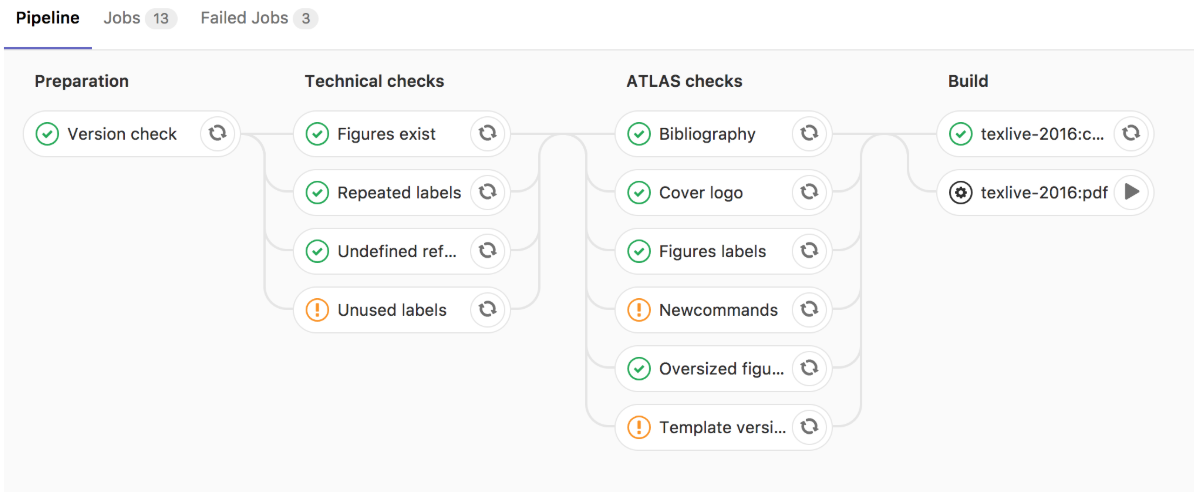
\includegraphics[width=0.9\textwidth]{editing_pipelines_1}
  \caption{Screenshot of the edit-pipelines.
    \GSnote[inline]{}{Expand caption. Explain that there are 4 stages in this image, with the preparation stage checking the version of the po-gitlab package, the second stage is ..., the third stage is ..., etc... This is explained in more detail in the note, so an abridged summary here is good.}}%
  \label{fig:edit-pipelines}
\end{figure}

\Cref{fig:edit-pipelines} presents an example of the edit-pipelines that consist of the following set of stages:
\begin{itemize}
\item \textbf{Preparation}: It consist of only one job that checks the current version of the \pogitlab package.

\item \textbf{Technical checks}: This stage includes checks related to \LaTeX: % chktex 13
  \begin{itemize}
  \item Figures exist: check if all figures used in the document are present in the repository or if any is missing.
  \item Files exist: check if all the \File{tex} files included in the document are present.
  \item Repeated commands: checks for repeated user-defined commands.
    It is not wise to use the same command for different purposes and can be an issue when generating captions for figures and tables for the ATLAS public pages.
  \item Repeated labels: checks for duplicate labels in all \File{tex} files.
  \item Undefined references: checks for undefined references.
  \item Unused labels: warnings of a \LaTeX\ label which has been defined but not used.
    Although this is not an issue it might point to something not being properly referenced.
  \end{itemize}

\item \textbf{ATLAS checks}: These are checks related to ATLAS rules and style:
  \begin{itemize}
  \item Bibliography: checks that the bibliography files are included.
  \item Cover logo: checks that the proper logo is being used in the ATLAS template.
  \item Figures labels: checks the ATLAS labels (e.g.\ \enquote{ATLAS Internal}) in the legends of figures depending on the type of document. \Cref{tab:labels} shows the different labels which are allowed and not allowed in different files.
  \item Oversized figures: checks for figures larger than \SI{2}{\mega\byte}.
  \item Preprint ID\@: checks that the preprint ID is included in the document.
  \item Template version: checks that the version of the ATLAS \LaTeX\ template is the latest one available.
  \item Title and Abstract: checks that no user-defined commands (i.e.\ non-\LaTeX\ commands) are being used in the title and in the abstract.
  \end{itemize}

\item \textbf{Build}: this stage builds the document itself. The PDF file of the document is not usually \GSnote{saved}{stored as an artifact} to avoid \GSnote{increase in size of the repository}{You can always store as an artifact, but mark it to expire in 24h... so this is a weird justification}.
However, a manual job (only run when \GSnote{requested}{who requests?}) can build the document and save the PDF file as an artifact for \GSnote{the}{a} user to download.
\end{itemize}

\begin{table}[htb]
  \centering
  \begin{tabular}{lll}\toprule
    Document type & Preliminary label & Internal label \\
    \midrule
    PAPER & Not allowed & Not allowed \\
    BOOK & Not allowed & Not allowed \\
    CONF & Allowed & Not allowed \\
    PUB & Allowed & Not allowed \\
    NOTE & Allowed & Allowed \\
    \bottomrule
  \end{tabular}
  \caption{Labels in legends that are allowed and not allowed in figures depending on the document type.
    The files and figures exist checks are needed because it is rather common to forget committing a new file or figure.
    \GSnote[inline]{}{I don't understand the caption. Please rephrase/clarify.}}%
  \label{tab:labels}
\end{table}

%------------------------------------------------------------------------------
\subsection{Paper submission}%
\label{sec:Paper_submission}

\GSnote{The GitLab’s CI}{The CI} also produces the required files for paper submission, using dedicated pipelines, similar to the editing ones.
These are referred to as \texttt{submit-pipelines} here.
A protected Git branch, named \texttt{PO-ready}, is created by default at the time of the setup of the paper repository.
When a paper is ready for submission, an editor should create a \enquote{Merge Request}
from the \texttt{Master} to the \texttt{PO-ready} branch.
When this request is accepted by a Physics Office officer, the paper submission pipelines are triggered.
In addition, any \IBnote{branch}{also tag?} created with a name of the form \texttt{PO-*} triggers the paper submission pipelines.
These pipelines have the previously described tests, but after at the build stage a flattening of the LaTeX document happens, with the following actions:

\begin{enumerate}
\item all the source files are merged into a single \LaTeX\ source file;
\item all the comments in the \LaTeX\ source file are removed;
\item all the figures are renamed following the convention required by the APS journals;
\item any directory structure is removed.
\end{enumerate}
The various actions are shown in \cref{fig:submit-pipelines}.

Furthermore, tarballs suitable for submission to arXiv and APS journals are created using \TeX{}Live \GSnote{2016 and 2017}{First time mentioning the version years.. need a section explaining when/why you pick specific versions to support}, respectively, and a tarball with the required files for the public webpage with plots and tables is created. These tarballs are created as GitLab artifacts and can be downloaded by the members of the Physics Office and editors. In the submission tarballs, the auxiliary material (figures and tables not for submission) are not included.

\begin{figure}[htb]
  \centering
  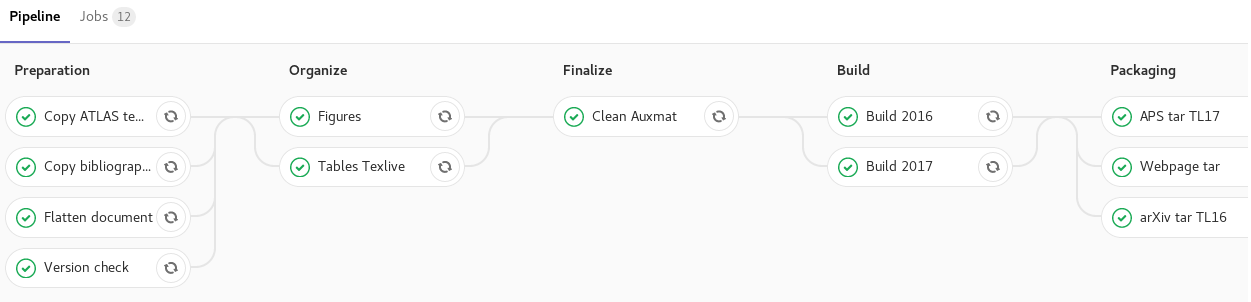
\includegraphics[width=0.9\textwidth]{editing_pipelines_2}
  \caption{Screenshot of submit-pipelines.
    \GSnote[inline]{}{Please expand caption more... you don't have any details of these stages in the text like you did with the edit-pipeline}}%
  \label{fig:submit-pipelines}
\end{figure}


